\documentclass[t]{beamer}

%%%%%%%%%%%%%%%%%%%%%%%%%%%%%%
% Packages
%%%%%%%%%%%%%%%%%%%%%%%%%%%%%%

\usepackage{geometry}              		 % 
\usepackage[dutch]{babel}                % Voor nederlandstalige hyphenatie (woordsplitsing)
\uselanguage{dutch}
\languagepath{dutch}
\usepackage{amsmath,amsthm}              % Uitgebreide wiskundige mogelijkheden
\usepackage{url}                         % Om url's te verwerken
\usepackage{graphicx,subfigure}          % Om figuren te kunnen verwerken
\usepackage{color}						 % Om kleuren in Inkscape figuren te kunnen weergeven
\usepackage[utf8]{inputenc}              % Om niet ascii karakters rechtstreeks te kunnen typen
\usepackage{float}                       % Om nieuwe float environments aan te maken. Ook optie H!
\usepackage[section]{placeins}			 % Om ervoor te zorgen dat floats binnen dezelfde section blijven
\usepackage{eurosym}                     % om het euro symbool te krijgen
\usepackage{textcomp}                    % Voor onder andere graden celsius
%\usepackage{fancyhdr}                    % Voor fancy headers en footers
\usepackage{parskip}                     % Om paragrafen met een verticale spatie ipv horizontaal te laten beginnen
\usepackage{multicol}
%\usepackage[plainpages=false]{hyperref}  % Om hyperlinks te hebben in het pdfdocument
\usepackage[absolute,overlay]{textpos}

%%%%%%%%%%%%%%%%%%%%%%%%%%%%%%
% Layout
%%%%%%%%%%%%%%%%%%%%%%%%%%%%%%
\usetheme{Frankfurt}
\AtBeginSection[]
{
  \begin{frame}
    \frametitle{Inhoud}
    \tableofcontents[currentsection]
  \end{frame}
}

%%%%%%%%%%%%%%%%%%%%%%%%%%%%%%
% Omgevingen
%%%%%%%%%%%%%%%%%%%%%%%%%%%%%%


%%%%%%%%%%%%%%%%%%%%%%%%%%%%%%
% Nieuwe commandos
%%%%%%%%%%%%%%%%%%%%%%%%%%%%%%

% De differentiaal operator
\newcommand{\diff}{\ensuremath{\mathrm{d}}}
\newcommand{\subsdiff}{\ensuremath{\mathrm{D}}}
\newcommand{\vardiff}{\ensuremath{\mathrm{\delta}}}

% Super en subscript
\newcommand{\supsc}[1]{\ensuremath{^{\text{#1}}}}   % Superscript in tekst
\newcommand{\subsc}[1]{\ensuremath{_{\text{#1}}}}   % Subscript in tekst

% Vectoren en matrices
\newcommand{\vt}[1]{\ensuremath{\boldsymbol{#1}}} % vector in juiste lettertype
\newcommand{\mx}[1]{\ensuremath{\mathsf{#1}}}	  % matrix in juiste lettertype

% Nieuw commando om iets te benadrukken en tegelijkertijd in de index te steken.
\newcommand{\begrip}[1]{\index{#1}\textbf{#1}\xspace}

% Graden celcius
\newcommand{\degC}{\ensuremath{^\circ \mathrm{C}}}


% nieuw commando om svg files dynamisch te updaten
\newcommand{\executeiffilenewer}[3]{%
\ifnum\pdfstrcmp{\pdffilemoddate{#1}}%
{\pdffilemoddate{#2}}>0%
{\immediate\write18{#3}}\fi%
}
% nieuw commando om. svg figuren in te voegen
% Gebruik: \includesvg{path/filename.svg}
\newcommand{\includesvg}[2][0]{%
\executeiffilenewer{#2.svg}{#2.pdf}%
{inkscape -z -C --file=#2.svg %
--export-pdf=#2.pdf --export-latex}%
\ifx#10
	\let\svgwidth\undefined
\else
	\def\svgwidth{#1}
\fi%
\input{#2.pdf_tex}%
\ifx \svgwidth\undefined
\else
	\let\svgwidth\undefined
\fi%
}

% nieuw commando om .fig figuren in te voegen
\newcommand{\includefig}[2][0]{%
\ifx#10
	\let\figwidth\undefined
\else
	\def\figwidth{#1}
\fi%
\input{#2.pdf_tex}%
\ifx \figwidth\undefined
\else
	\let\figwidth\undefined
\fi%
}

\graphicspath{{../fig/controlevolumes/}}

\title{Fluïdummechanica}
\subtitle{Hydrostatica}
\author{Brecht Baeten\inst{1}}
\institute{
	\inst{1}%
  		KU Leuven, Technologie campus Diepenbeek, e-mail: brecht.baeten@kuleuven.be
}
\date{\today}

\begin{document}

	\frame{\titlepage}
	\section{Inleiding}
		\begin{frame}
		
			\frametitle{Voorbeeld}
			\center
    		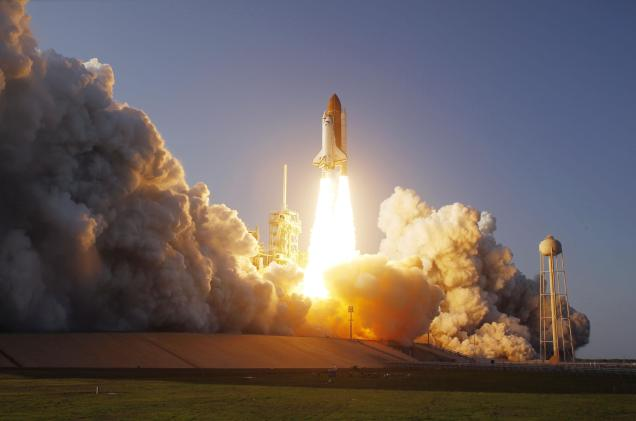
\includegraphics[height=0.8\textheight]{../fig/controlevolumes/space_shuttle.jpg}\\
			\footnotesize{Bron: http://www.nasa.gov/}
			
  		\end{frame}
%%%%%%%%%%%%%%%%%%%%%%%%%%%%%%%%%%%%%%%%%%%%%%%%%%%%%%%%%%%%%%%%%%%%%%%%%%%
  	\section{Controle massa's}	
  		\begin{frame}
			\frametitle{Mechanica}
			\pause 
			Behoud van massa
			\begin{equation}
				\frac{\diff m}{\diff t} = 0
			\end{equation}
			
			\pause 			
			Behoud van impuls
			\begin{equation}
				\frac{\diff \vt{P}}{\diff t} = \vt{F}
			\end{equation}
			
			\pause 
			Behoud van energie
			\begin{equation}
				\frac{\diff E}{\diff t} = \dot{Q}-\dot{W}
			\end{equation}
  		\end{frame}
%%%%%%%%%%%%%%%%%%%%%%%%%%%%%%%%%%%%%%%%%%%%%%%%%%%%%%%%%%%%%%%%%%%%%%%%%%%
  	\section{Controle volumes}	
  		\begin{frame}
			\frametitle{Controlevolume}
			\vspace{1cm}
			\center
			\includesvg{../fig/controlevolumes/Controlevolume_met_stroomlijnen}
  		\end{frame}
%%%%%%%%%%%%%%%%%%%%%%%%%%%%%%%%%%%%%%%%%%%%%%%%%%%%%%%%%%%%%%%%%%%%%%%%%%%
  		\begin{frame}
			\frametitle{Behoud van massa}
			\vspace{2cm}
			\begin{equation}
				\left[
					\begin{array}{c}
						\mbox{De verandering} \\ \mbox{van massa in} \\ \mbox{het controlevolume}
					\end{array}
				\right]
				+
				\left[
					\begin{array}{c}
						\mbox{De netto} \\ \mbox{massastroom uit} \\ \mbox{het controlevolume}
					\end{array}
				\right]
				= 0
				\label{eqn:controlevolume,behoud van massa,woorden}
			\end{equation}
		\end{frame}	
%%%%%%%%%%%%%%%%%%%%%%%%%%%%%%%%%%%%%%%%%%%%%%%%%%%%%%%%%%%%%%%%%%%%%%%%%%%
		\begin{frame}
			\frametitle{Massastroom}
			\vspace{1cm}
			\center
			\includesvg{../fig/controlevolumes/massastroom}
  		\end{frame}
%%%%%%%%%%%%%%%%%%%%%%%%%%%%%%%%%%%%%%%%%%%%%%%%%%%%%%%%%%%%%%%%%%%%%%%%%%%
  		\begin{frame}
  			\frametitle{Massastroom}
  			\begin{equation}
				\Delta m = \rho \Delta x_{\perp} \diff A
			\end{equation}
  			
  			\pause
  			\begin{equation}
				\Delta m = \rho v_{\perp} \Delta t \diff A
			\end{equation}
			
			\pause
  			\begin{equation}
				\frac{\Delta m}{\Delta t} = \rho v_{\perp} \diff A
			\end{equation}
			
			\pause
			\begin{equation}
				\diff \dot{m}  = \rho v_{\perp} \diff A
				\label{eqn:massastroom}
			\end{equation}
  		\end{frame}
%%%%%%%%%%%%%%%%%%%%%%%%%%%%%%%%%%%%%%%%%%%%%%%%%%%%%%%%%%%%%%%%%%%%%%%%%%%
  		\begin{frame}
			\frametitle{Behoud van impuls}
			\vspace{1.5cm}
			\begin{equation}
				\left[
					\begin{array}{c}
						\mbox{De verandering} \\ \mbox{van impuls} \\ \mbox{in het}  \\ \mbox{controlevolume}
					\end{array}
				\right]
				+
				\left[
					\begin{array}{c}
						\mbox{De netto} \\ \mbox{impulsstroom} \\ \mbox{uit het} \\ \mbox{controlevolume}
					\end{array}
				\right]
				=
				\left[
					\begin{array}{c}
						\mbox{De totale} \\ \mbox{kracht} \\ \mbox{op het} \\ \mbox{controlevolume}
					\end{array}
				\right]
				\label{eqn:controlevolume,behoud van massa,woorden}
			\end{equation}
		\end{frame}	
%%%%%%%%%%%%%%%%%%%%%%%%%%%%%%%%%%%%%%%%%%%%%%%%%%%%%%%%%%%%%%%%%%%%%%%%%%%
  		\begin{frame}
			\frametitle{Behoud van energie}
			\vspace{1.3cm}
			\begin{equation}
				\left[
					\begin{array}{c}
						\mbox{De verandering} \\ \mbox{van energie} \\ \mbox{in het} \\ \mbox{controlevolume}
					\end{array}
				\right]
				+
				\left[
					\begin{array}{c}
						\mbox{De netto} \\ \mbox{energiestroom} \\ \mbox{uit het} \\ \mbox{controlevolume}
					\end{array}
				\right]
				=
				\left[
					\begin{array}{c}
						\mbox{De warmtesroom} \\ \mbox{toegevoegd en} \\   \mbox{arbeidsstroom} \\ \mbox{onttrokken aan } \\ \mbox{het controlevolume}
					\end{array}
				\right]
				\label{eqn:controlevolume,behoud van massa,woorden}
			\end{equation}
		\end{frame}	
%%%%%%%%%%%%%%%%%%%%%%%%%%%%%%%%%%%%%%%%%%%%%%%%%%%%%%%%%%%%%%%%%%%%%%%%%%%
\end{document}